%% fig_descent.tex   (generated by make_round11.py; do not edit by hand)
%% The web of Weil families linked by descent and scalar extension.
\documentclass[tikz,border=8pt]{standalone}
\usepackage{amsmath,amssymb}
\usetikzlibrary{arrows.meta,calc,decorations.pathreplacing}
%% palette.tex -- shared colour definitions for the figures
\definecolor{PInk}{RGB}{26,32,44}
\definecolor{PBlue}{RGB}{37,82,139}
\definecolor{PTeal}{RGB}{23,127,125}
\definecolor{POchre}{RGB}{193,138,44}
\definecolor{PClay}{RGB}{178,74,58}
\definecolor{PSlate}{RGB}{108,122,137}
\definecolor{PViolet}{RGB}{110,86,150}
\definecolor{WBlue}{RGB}{223,234,246}
\definecolor{WTeal}{RGB}{220,238,236}
\definecolor{WOchre}{RGB}{250,240,218}
\definecolor{WClay}{RGB}{247,229,224}
\definecolor{WSlate}{RGB}{238,241,244}
\definecolor{PMag}{RGB}{158,58,110}
\definecolor{PGrass}{RGB}{62,124,66}
\definecolor{PAmber}{RGB}{214,112,38}
\definecolor{PIndigo}{RGB}{58,64,140}
\definecolor{PRule}{RGB}{176,186,197}

%% shared macros so the standalone figures match the paper
\providecommand{\QQ}{\mathbb{Q}}
\providecommand{\ZZ}{\mathbb{Z}}
\providecommand{\RR}{\mathbb{R}}
\providecommand{\CC}{\mathbb{C}}
\providecommand{\PP}{\mathbb{P}}
\providecommand{\Kx}{K^{\times}}
\providecommand{\HW}{W}
\providecommand{\Nm}{\mathrm{N}}
\providecommand{\Hdg}{\mathrm{Hdg}}
\providecommand{\NS}{\mathrm{NS}}
\providecommand{\cA}{\mathcal{A}}
\providecommand{\cD}{\mathcal{D}}
\providecommand{\cF}{\mathcal{F}}
\providecommand{\cP}{\mathcal{P}}
\providecommand{\cO}{\mathcal{O}}
\providecommand{\cQ}{\mathcal{Q}}
\providecommand{\bbar}[1]{\overline{#1}}
\providecommand{\ch}{\operatorname{ch}}
\providecommand{\End}{\mathrm{End}}

\begin{document}
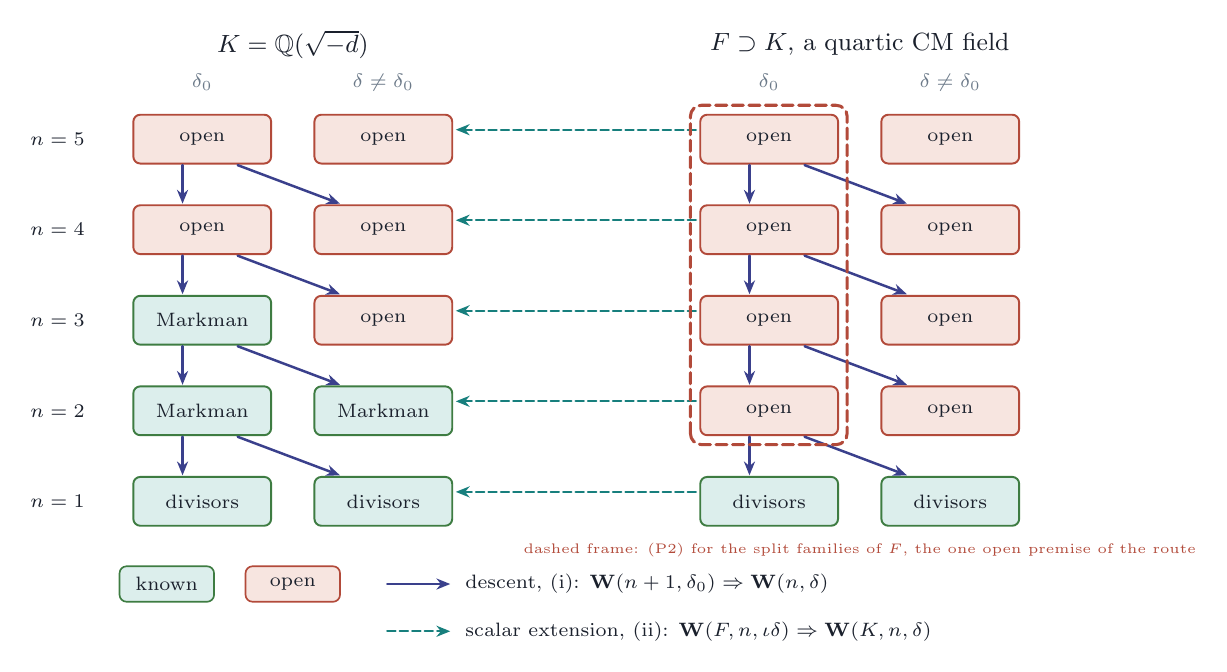
\begin{tikzpicture}[x=1cm,y=1cm,line join=round,line cap=round,
  font=\small,text=PInk]
  \node[draw=PGrass,fill=WTeal,rounded corners=2.5pt,inner sep=3pt,line width=0.70pt,align=center,minimum width=1.75cm,minimum height=0.62cm,font=\scriptsize] at (1.00,0.00) {divisors};
  \node[draw=PGrass,fill=WTeal,rounded corners=2.5pt,inner sep=3pt,line width=0.70pt,align=center,minimum width=1.75cm,minimum height=0.62cm,font=\scriptsize] at (8.20,0.00) {divisors};
  \node[draw=PGrass,fill=WTeal,rounded corners=2.5pt,inner sep=3pt,line width=0.70pt,align=center,minimum width=1.75cm,minimum height=0.62cm,font=\scriptsize] at (3.30,0.00) {divisors};
  \node[draw=PGrass,fill=WTeal,rounded corners=2.5pt,inner sep=3pt,line width=0.70pt,align=center,minimum width=1.75cm,minimum height=0.62cm,font=\scriptsize] at (10.50,0.00) {divisors};
  \node[text=PInk,inner sep=1pt,align=center,font=\scriptsize,anchor=east] at (-0.45,0.00) {$n=1$};
  \node[draw=PGrass,fill=WTeal,rounded corners=2.5pt,inner sep=3pt,line width=0.70pt,align=center,minimum width=1.75cm,minimum height=0.62cm,font=\scriptsize] at (1.00,1.15) {Markman};
  \node[draw=PClay,fill=WClay,rounded corners=2.5pt,inner sep=3pt,line width=0.70pt,align=center,minimum width=1.75cm,minimum height=0.62cm,font=\scriptsize] at (8.20,1.15) {open};
  \node[draw=PGrass,fill=WTeal,rounded corners=2.5pt,inner sep=3pt,line width=0.70pt,align=center,minimum width=1.75cm,minimum height=0.62cm,font=\scriptsize] at (3.30,1.15) {Markman};
  \node[draw=PClay,fill=WClay,rounded corners=2.5pt,inner sep=3pt,line width=0.70pt,align=center,minimum width=1.75cm,minimum height=0.62cm,font=\scriptsize] at (10.50,1.15) {open};
  \node[text=PInk,inner sep=1pt,align=center,font=\scriptsize,anchor=east] at (-0.45,1.15) {$n=2$};
  \node[draw=PGrass,fill=WTeal,rounded corners=2.5pt,inner sep=3pt,line width=0.70pt,align=center,minimum width=1.75cm,minimum height=0.62cm,font=\scriptsize] at (1.00,2.30) {Markman};
  \node[draw=PClay,fill=WClay,rounded corners=2.5pt,inner sep=3pt,line width=0.70pt,align=center,minimum width=1.75cm,minimum height=0.62cm,font=\scriptsize] at (8.20,2.30) {open};
  \node[draw=PClay,fill=WClay,rounded corners=2.5pt,inner sep=3pt,line width=0.70pt,align=center,minimum width=1.75cm,minimum height=0.62cm,font=\scriptsize] at (3.30,2.30) {open};
  \node[draw=PClay,fill=WClay,rounded corners=2.5pt,inner sep=3pt,line width=0.70pt,align=center,minimum width=1.75cm,minimum height=0.62cm,font=\scriptsize] at (10.50,2.30) {open};
  \node[text=PInk,inner sep=1pt,align=center,font=\scriptsize,anchor=east] at (-0.45,2.30) {$n=3$};
  \node[draw=PClay,fill=WClay,rounded corners=2.5pt,inner sep=3pt,line width=0.70pt,align=center,minimum width=1.75cm,minimum height=0.62cm,font=\scriptsize] at (1.00,3.45) {open};
  \node[draw=PClay,fill=WClay,rounded corners=2.5pt,inner sep=3pt,line width=0.70pt,align=center,minimum width=1.75cm,minimum height=0.62cm,font=\scriptsize] at (8.20,3.45) {open};
  \node[draw=PClay,fill=WClay,rounded corners=2.5pt,inner sep=3pt,line width=0.70pt,align=center,minimum width=1.75cm,minimum height=0.62cm,font=\scriptsize] at (3.30,3.45) {open};
  \node[draw=PClay,fill=WClay,rounded corners=2.5pt,inner sep=3pt,line width=0.70pt,align=center,minimum width=1.75cm,minimum height=0.62cm,font=\scriptsize] at (10.50,3.45) {open};
  \node[text=PInk,inner sep=1pt,align=center,font=\scriptsize,anchor=east] at (-0.45,3.45) {$n=4$};
  \node[draw=PClay,fill=WClay,rounded corners=2.5pt,inner sep=3pt,line width=0.70pt,align=center,minimum width=1.75cm,minimum height=0.62cm,font=\scriptsize] at (1.00,4.60) {open};
  \node[draw=PClay,fill=WClay,rounded corners=2.5pt,inner sep=3pt,line width=0.70pt,align=center,minimum width=1.75cm,minimum height=0.62cm,font=\scriptsize] at (8.20,4.60) {open};
  \node[draw=PClay,fill=WClay,rounded corners=2.5pt,inner sep=3pt,line width=0.70pt,align=center,minimum width=1.75cm,minimum height=0.62cm,font=\scriptsize] at (3.30,4.60) {open};
  \node[draw=PClay,fill=WClay,rounded corners=2.5pt,inner sep=3pt,line width=0.70pt,align=center,minimum width=1.75cm,minimum height=0.62cm,font=\scriptsize] at (10.50,4.60) {open};
  \node[text=PInk,inner sep=1pt,align=center,font=\scriptsize,anchor=east] at (-0.45,4.60) {$n=5$};
  \draw[PIndigo,line width=0.90pt,-{Stealth[length=5pt,width=4pt]}] (0.75,0.82) to (0.75,0.33);
  \draw[PIndigo,line width=0.90pt,-{Stealth[length=5pt,width=4pt]}] (1.45,0.82) to (2.75,0.33);
  \draw[PIndigo,line width=0.90pt,-{Stealth[length=5pt,width=4pt]}] (7.95,0.82) to (7.95,0.33);
  \draw[PIndigo,line width=0.90pt,-{Stealth[length=5pt,width=4pt]}] (8.65,0.82) to (9.95,0.33);
  \draw[PIndigo,line width=0.90pt,-{Stealth[length=5pt,width=4pt]}] (0.75,1.97) to (0.75,1.48);
  \draw[PIndigo,line width=0.90pt,-{Stealth[length=5pt,width=4pt]}] (1.45,1.97) to (2.75,1.48);
  \draw[PIndigo,line width=0.90pt,-{Stealth[length=5pt,width=4pt]}] (7.95,1.97) to (7.95,1.48);
  \draw[PIndigo,line width=0.90pt,-{Stealth[length=5pt,width=4pt]}] (8.65,1.97) to (9.95,1.48);
  \draw[PIndigo,line width=0.90pt,-{Stealth[length=5pt,width=4pt]}] (0.75,3.12) to (0.75,2.63);
  \draw[PIndigo,line width=0.90pt,-{Stealth[length=5pt,width=4pt]}] (1.45,3.12) to (2.75,2.63);
  \draw[PIndigo,line width=0.90pt,-{Stealth[length=5pt,width=4pt]}] (7.95,3.12) to (7.95,2.63);
  \draw[PIndigo,line width=0.90pt,-{Stealth[length=5pt,width=4pt]}] (8.65,3.12) to (9.95,2.63);
  \draw[PIndigo,line width=0.90pt,-{Stealth[length=5pt,width=4pt]}] (0.75,4.27) to (0.75,3.78);
  \draw[PIndigo,line width=0.90pt,-{Stealth[length=5pt,width=4pt]}] (1.45,4.27) to (2.75,3.78);
  \draw[PIndigo,line width=0.90pt,-{Stealth[length=5pt,width=4pt]}] (7.95,4.27) to (7.95,3.78);
  \draw[PIndigo,line width=0.90pt,-{Stealth[length=5pt,width=4pt]}] (8.65,4.27) to (9.95,3.78);
  \draw[PTeal,line width=0.80pt,-{Stealth[length=5pt,width=4pt]},dash pattern=on 3pt off 1.5pt] (7.27,0.12) to (4.22,0.12);
  \draw[PTeal,line width=0.80pt,-{Stealth[length=5pt,width=4pt]},dash pattern=on 3pt off 1.5pt] (7.27,1.27) to (4.22,1.27);
  \draw[PTeal,line width=0.80pt,-{Stealth[length=5pt,width=4pt]},dash pattern=on 3pt off 1.5pt] (7.27,2.42) to (4.22,2.42);
  \draw[PTeal,line width=0.80pt,-{Stealth[length=5pt,width=4pt]},dash pattern=on 3pt off 1.5pt] (7.27,3.57) to (4.22,3.57);
  \draw[PTeal,line width=0.80pt,-{Stealth[length=5pt,width=4pt]},dash pattern=on 3pt off 1.5pt] (7.27,4.72) to (4.22,4.72);
  \node[text=PInk,inner sep=1pt,align=center,font=\small] at (2.15,5.80) {$K=\QQ(\sqrt{-d})$};
  \node[text=PInk,inner sep=1pt,align=center,font=\small] at (9.35,5.80) {$F\supset K$, a quartic CM field};
  \node[text=PSlate,inner sep=1pt,align=center,font=\scriptsize] at (1.00,5.32) {$\delta_{0}$};
  \node[text=PSlate,inner sep=1pt,align=center,font=\scriptsize] at (3.30,5.32) {$\delta\neq\delta_{0}$};
  \node[text=PSlate,inner sep=1pt,align=center,font=\scriptsize] at (8.20,5.32) {$\delta_{0}$};
  \node[text=PSlate,inner sep=1pt,align=center,font=\scriptsize] at (10.50,5.32) {$\delta\neq\delta_{0}$};
  \draw[PClay,line width=1.1pt,rounded corners=4pt,dash pattern=on 4pt off 2pt] (7.20,0.72) rectangle (9.19,5.03);
  \node[text=PClay,inner sep=1pt,align=center,font=\tiny] at (9.35,-0.62) {dashed frame: (P2) for the split families of $F$, the one open premise of the route};
  \node[draw=PGrass,fill=WTeal,rounded corners=2.5pt,inner sep=3pt,line width=0.60pt,align=center,minimum width=1.20cm,minimum height=0.45cm,font=\scriptsize] at (0.55,-1.05) {known};
  \node[draw=PClay,fill=WClay,rounded corners=2.5pt,inner sep=3pt,line width=0.60pt,align=center,minimum width=1.20cm,minimum height=0.45cm,font=\scriptsize] at (2.15,-1.05) {open};
  \draw[PIndigo,line width=0.90pt,-{Stealth[length=5pt,width=4pt]}] (3.35,-1.05) to (4.15,-1.05);
  \node[text=PInk,inner sep=1pt,align=center,font=\scriptsize,anchor=west] at (4.30,-1.05) {descent, (i): $\mathbf{W}(n+1,\delta_{0})\Rightarrow\mathbf{W}(n,\delta)$};
  \draw[PTeal,line width=0.80pt,-{Stealth[length=5pt,width=4pt]},dash pattern=on 3pt off 1.5pt] (3.35,-1.65) to (4.15,-1.65);
  \node[text=PInk,inner sep=1pt,align=center,font=\scriptsize,anchor=west] at (4.30,-1.65) {scalar extension, (ii): $\mathbf{W}(F,n,\iota\delta)\Rightarrow\mathbf{W}(K,n,\delta)$};
\end{tikzpicture}
\end{document}
